\subsection{Методы потокового распределения (online partitioning}
В этой секции будут использоваться следующие обозначения:  $P^t$ - распределение вершин по шардам (состояние шардов) в момент времени t, $P^t(i)$ - состояние шарда i в момент времени t, $v$ - некая вершина, $N(v)$ - соседи вершины v, $C$ - максимальная вместимость шарда.

\subsubsection{Балансировочные}
Простейшие методы распределения новых вершин, не решающие задачу, поставленную выше, а предназначенные просто для равномерного распределения данных по шардам. Стоят упоминания, так как используются в последующих методах, а также могут быть использованы на начальных этапах.

Всего их три:

\begin{enumerate}
    \item Поочерёдное — распределение записей по шардам по очереди. По сути round-robin.
    \item Групповое — записи на шарды загружаются сразу большим набором исходя из ожидаемого количества и следуемого из этого количества записей на каждом шарде.
    \item Случайное/Псевдослучайное — абсолютно или частично случайное распределение вершин по шардам.
\end{enumerate}

\subsubsection{Хеширование}
Технически попадает в группу методов описанную выше, конкретно в псевдослучайные, но, в отличии от них, активно используется сам по себе, а не как начальный этап или основа для других методов.

Заключается в использовании хеш-функции на каких-либо атрибутах вершин. Для лучшего решения задачи можно хешировать атрибуты, которые естественным образом совпадают у близких вершин, например, географические. 

Используется, например, в ArangoDB \cite{ArangoDBRepo} (Файл arangod\textbackslash Sharding\textbackslash ShardingStrategyDefault.cpp, метод getResponsibleShard), где хеширование применяется дважды: сначала хешируются атрибуты, после чего хешируется полученный хеш. Примечание: это не связано с алгоритмом двойного хеширования для решения коллизий, коллизии в понимании этого алгоритма не случаются при распредении вершин по шардам.

\subsubsection{Streaming Graph Partitioning}
Потоковое распределение графов \cite{SGP} (англ. Streaming Graph Partitioning) - алгоритм, а точнее набор алгоритмов, для распределения вершин графа, которые приходят "потоком" по одной или небольшими наборами (оба варианта простейшим образом можно переводить друг в друга, поэтому далее их разделения не будет), с использованием эвристик для оценки насколько новая вершина подходит и штрафов, чтобы не избежать загрузки большинства вершин на один шард.

Метод учитывает три возможных варианта организации потока:
\begin{enumerate}
    \item Случайное - вершины графа приходят в случайном порядке. 
    \item Обход в ширину (BFS) - первая вершина выбирается случайно, каждая следующая приходит согласно обходу в ширину.
    \item Обход в глубину (DFS) - аналогично обходу в ширину, но согласно обходу в глубину.
\end{enumerate}

Для балансироваки распределения в эвристиках используются следующие весовые функции:
\begin{enumerate}
    \item $w(t,i)=1$ - без взвешивания.
    \item $w(t,i)=1-\frac{|P^t(i)|}{C}$ - линейный вес.
    \item $w(t,i)=1-e^{|P^t(i)-C|}$ - экспоненциальный вес.
\end{enumerate}

Предлагаемые эвристики:
\begin{enumerate}
    \item Балансировка - распределение по шардам с наименьшим кол-вом вершин.
    \item Групповая (Chunking) - описанное выше групповое распределение
    \item (Вес) Детерминированная жадная (DG): 
    \begin{equation*}
        ind=arg max_{i\in k}\{|P^t(i)\cap N(v)|w(t,i)\}
    \end{equation*}где $w(t,i)$ - одна из описанных выше весовых функций.
    \item (Вес) Случайная жадная (RG): выбор шарда происходит следующего распределения
    \begin{equation*}
        Pr(i)=\frac{|P^t(i)\cap N(v)|w(t,i)}{Z}
    \end{equation*}где $w(t,i)$ - одна из описанных выше весовых функций, a $Z$ - нормализующая константа. В оригинальной статье отмечается, что случайная эвристика рассматривается только потому что она может лучше работать в худшем случае организации потока.
    \item (Вес) Треугольники:
    \begin{equation*}
        ind=arg max_{i\in k}\{\frac{|E(P^t(u)\cap N(v),(P^t(u)\cap N(v))|}{\binom{|P^t(u)\cap N(v)|}{2}}\}w(t,i)
    \end{equation*}где $w(t,i)$ - одна из описанных выше весовых функций, $E(S,T)$ - набор рёбер между наборами верши S и T. Идея заключается в сохранении наибольшего кол-ва треугольников на шарде, что, очевидно, приведёт к хорошей связности на нём.
    \item Балансировка большого
    При возможности определять степень вершины и насколько она велика относительно всего графа распределять вершины с большой степенью балансировкой, а с маленькой DG. 
\end{enumerate}

Дальнейшие эвристики предполагают буферизацию:
\begin{enumerate}\addtocounter{enumi}{6}
    \item Предпочтение большому - начать с вершин больших степеней, использовать балансировку большого.
    \item Избегание большого - распределить жадным алгоритмом вершины малых степеней, когда останутся только вершины с большими степенями распределить их DG.
    \item Жадный EvoCut - использовать EvoCut \cite{EvoCut} на подграфе в буфере, найти малые множества  (англ. nibbles) с хорошей проводимостью и распределить их по шардам DG.
\end{enumerate}

Метод в первую очередь направлен на графы соц.сетей, где и используется.

\textbf{Сравнение эвристик}

Для оценки качества определения считается процент среднего улучшения по следующей формуле:
\begin{equation*}
    \text{gain} = \frac{\text{edges\_cut\_random} - \text{edges\_cut\_heuristic}}{\text{edges\_cut\_random} - \text{edges\_cut\_METIS}} \times 100\%
\end{equation*}

Где edges\_cut\_random - кол-во ребёр между шардами при хешировании, edges\_cut\_heuristic - кол-во рёбер между шардами в эксперименте, а edges\_cut\_METIS количество рёбер между шардами при использовании METIS.

Метод и его производный Fennel \cite{Fennel} используются в соц. сетях и рекомендательных системах, на графах которых и будет проводиться сравнение. 

Сравнение эвристик представлено в следующей таблице:
\begin{table}[H]
\centering
\begin{tabular}{|c|l|c|c|c|}
\hline
Сокращение & Эвристика & \textit{BFS} & \textit{DFS} & \textit{Случайное} \\
\hline
B & Балансировка & -1.5 & -1.3 & -0.2 \\ \hline
C & Групповое & 37.6 & 35.7 & 0.7 \\ \hline
H & Хеширование & -1.9 & -2.1 & -1.7 \\ \hline
DG & Детерминированная жадная & 57.7 & 54.7 & 45.4 \\ \hline
RG & Случайная жадная & 45.5 & 44.9 & 38.7 \\ \hline
T & Треугольники & 49.7 & 48.4 & 40.2 \\ \hline
LDG & Лин. Дет. жадная & 76.0 & 73.0 & 75.3 \\ \hline
LRG & Лин. Случ. жадная & 46.4 & 44.9 & 39.1 \\ \hline
LT & Лин. Треугольники & 55.4 & 54.6 & 49.3 \\ \hline
EDG & Эксп. Дет. жадная & 59.4 & 56.2 & 47.5 \\ \hline
ERG & Эксп. Случ. жадная & 45.6 & 45.6 & 38.8 \\ \hline
ET & Эксп. Треугольники & 50.7 & 49.3 & 41.6 \\ \hline
BB & Балансировка большого & 67.8 & 68.5 & 63.3 \\ \hline
PB & Предпочтение большому & -9.5 & -18.6 & -23.1 \\ \hline
AB & Избегание большого & -27.3 & -38.6 & -46.4 \\ \hline
GE & Жадный EvoCut & 60.3 & 58.6 & 43.1 \\
\hline
\end{tabular}
\caption{Среднее улучшение каждой эвристики по всем наборам данных и размерам партиций \cite{SGP}}
\end{table}

\begin{center}
    \centering
    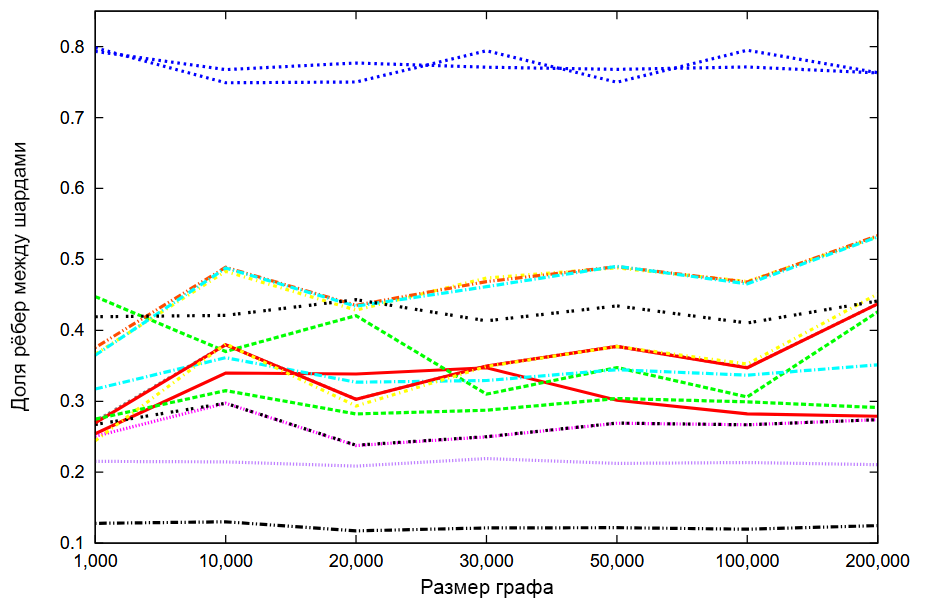
\includegraphics[width=.7\linewidth]{extras/SGP_perf.png}
    \captionof{figure}{Визуализация доли рёбер между шардами для 4 шардов с порядком BFS. Нижняя лития - METIS, предпоследняя нижняя - Лин. Дет. жадная \cite{SGP}}
    \label{fig:prplot}
\end{center}

Как можно увидеть по таблице и графику выше LDG даёт наилучшие результаты. 

\subsubsection{Fennel алгоритм}
Fennel алгоритм \cite{Fennel} - модификация потокового распределения графов.

Модификация заключается в определении так называемой объективной функции k-распределения $g(P)$, значение которой должно макисмально увеличиться при распределении новой вершины. По своей сути функция является эвристикой метода потокового распределения графов.

Опуская детали вывода функции описанные в оригинальной статье объективная функция k-распределения имеет следующий вид:

\begin{equation*}
    g(P)=\sum_{i=1}^k[e(S_i,S_i) - p\binom{|S_i|}{2}]
\end{equation*}
где $p=2\alpha=m\frac{k^{\gamma-1}}{n^\gamma}$, $1\le\gamma\le 2$.

Несмотря на относительную громоздкость самой функции, расчёт всех её вариантов не требуется, так как нужно найти максимальное $\delta g(v,S_i)=g(S_1,S_2...,S_i\cup v,...S_k)-g(S_1,S_2...S_k)$ для $i\in \{1...k\}$, притом что все $g(S_1,S_2...S_k)$ и $e(S_j,S_j) - p\binom{|S_j|}{2}$ были найдены при заносе предыдущих вершин. Также, очевидно, каждое $g(S_1,S_2...,S_i\cup v,...S_k)$ может быть вычислено на соответствующем шарде, если он способен на вычисления, что позволяет распараллелить все расчёты. 

\textbf{Балансировка}

Стоит отдельно упомянуть балансировку, так как алгоритм в "сыром" виде совсем не гарантирует хорошую балансировку, а при $\gamma = 1$, когда алгоритм сводится к отправлению вершин в шард с наибольшим числом её соседей, вообще имеет тенденцию к плохой балансировке.

Поэтому также предложена надстройка, позоволяющая гарантировать балансировку для $\rho = \tau$. Она заключается в изначальном отметании шардов, добавление вершины на которую превысит эту нагрузку, то есть таких шардов, где $|S_i\cup v| > \tau\frac{n}{k}$.

\textbf{Сравнение с другими методами по качеству}

Ниже предоставлены сравнения результатов работы алгоритма с другими эвристиками при $\gamma = \frac{3}{2}$ и $\tau=1.1$.

\begin{table}[H]
\centering
\begin{tabular}{|c|c|c|c|c|}
\hline
 & \multicolumn{2}{c|}{BFS} & \multicolumn{2}{c|}{Random} \\
\hline
Метод & $\lambda$ & $\rho$ & $\lambda$ & $\rho$ \\
\hline
H & 96.9\% & 1.01 & 96.9\% & 1.01 \\
B & 97.3\% & 1.00 & 96.8\% & 1.00 \\
LDG & 34\% & 1.01 & 40\% & 1.00 \\
EDG & 39\% & 1.04 & 48\% & 1.01 \\
T & 61\% & 2.11 & 78\% & 1.01 \\
LT & 63\% & 1.23 & 78\% & 1.10 \\
ET & 64\% & 1.05 & 79\% & 1.01 \\
\hline
Fennel & 14\% & 1.10 & 14\% & 1.02 \\
METIS & 8\% & 1.00 & 8\% & 1.02 \\
\hline
\end{tabular}
\caption{Качество работы различных методов на графе amazon0312 ($k=32$) \cite{Fennel}}
\end{table}

\begin{table}[H]
\centering
\begin{tabular}{|c|c|c|c|c|c|}
\hline
$m$ & $k$ & \multicolumn{2}{c|}{Fennel} & \multicolumn{2}{c|}{METIS} \\
\cline{3-6}
 & & $\lambda$ & $\rho$ & $\lambda$ & $\rho$ \\
\hline
7\,185\,314 & 4 & 62.5\% & 1.04 & 65.2\% & 1.02 \\
6\,714\,510 & 8 & 82.2\% & 1.04 & 81.5\% & 1.02 \\
6\,483\,201 & 16 & 92.9\% & 1.01 & 92.2\% & 1.02 \\
6\,364\,819 & 32 & 96.3\% & 1.00 & 96.2\% & 1.02 \\
6\,308\,013 & 64 & 98.2\% & 1.01 & 97.9\% & 1.02 \\
6\,279\,566 & 128 & 98.4\% & 1.02 & 98.8\% & 1.02 \\
\hline
\end{tabular}
\caption{Результаты Fennel и METIS, усреднённые по 5 случайным графам, сгенерированным по модели HP(5\,000, k, 0.8, 0.5) \cite{Fennel}.}
\end{table}

\textbf{Сравнение с другими методами по времени}

\begin{table}[H]
\centering
\begin{tabular}{|c|c|c|c|c|c|c|}
\hline
 & \multicolumn{2}{c|}{Fennel} & \multicolumn{2}{c|}{LDG} & \multicolumn{2}{c|}{METIS} \\
\hline
Кластеров ($k$) & $\lambda$ & $\rho$ & $\lambda$ & $\rho$ & $\lambda$ & $\rho$ \\
\hline
2 & 6.8\% & 1.1 & 34.3\% & 1.04 & 11.98\% & 1.02 \\
4 & 29\% & 1.1 & 55.0\% & 1.07 & 24.39\% & 1.03 \\
8 & 48\% & 1.1 & 66.4\% & 1.10 & 35.96\% & 1.03 \\
\hline
\end{tabular}
\caption{Результаты работы методов при распределении графа Twitter ($\approx$1.5 млрд рёбер). Распределение через Fennel и LDG заняло \cite{Fennel}.}
\end{table}

\begin{table}[H]
\centering
\begin{tabular}{|c|c|c|c|c|}
\hline
 & \multicolumn{2}{c|}{Время выполнения [с]} & \multicolumn{2}{c|}{Коммуникация [МБ]} \\
\hline
Кластеров ($k$) & Hash & Fennel & Hash & Fennel \\
\hline
4 & 32.27 & 25.49 & 321.41 & 196.9 \\
8 & 17.26 & 15.14 & 285.35 & 180.02 \\
16 & 10.64 & 9.05 & 222.28 & 148.67 \\
\hline
\end{tabular}
\caption{Средняя длительность шага и средний объем данных, передаваемых за шаг при выполнении \cite{Fennel}}
\end{table}